\documentclass{standalone}
\usepackage{tikz}
\usetikzlibrary{patterns, positioning}


\begin{document}
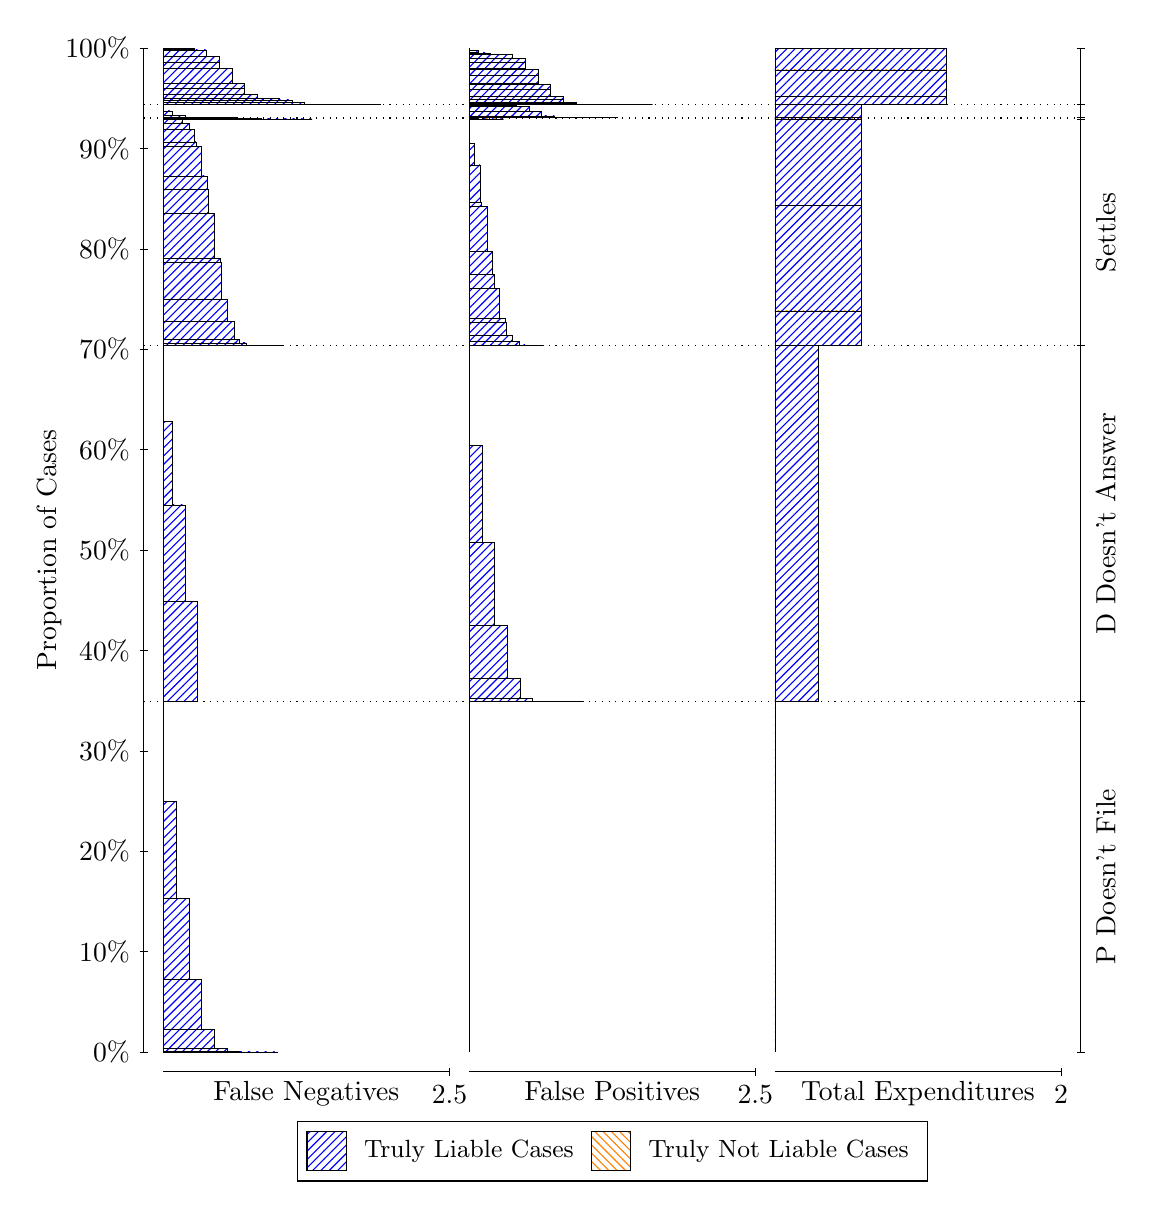
\begin{tikzpicture}
\draw[black, very thin] (1.5,1.75) -- (1.5,14.5);
\node[rotate=90, text=black, anchor=center] at (0.3, 8.125) {Proportion of Cases};
\draw[black, very thin] (1.45,1.75) -- (1.55,1.75);
\node[text=black, anchor=east] at (1.45, 1.75) {0\%};
\draw[black, very thin] (1.45,3.025) -- (1.55,3.025);
\node[text=black, anchor=east] at (1.45, 3.025) {10\%};
\draw[black, very thin] (1.45,4.3) -- (1.55,4.3);
\node[text=black, anchor=east] at (1.45, 4.3) {20\%};
\draw[black, very thin] (1.45,5.575) -- (1.55,5.575);
\node[text=black, anchor=east] at (1.45, 5.575) {30\%};
\draw[black, very thin] (1.45,6.85) -- (1.55,6.85);
\node[text=black, anchor=east] at (1.45, 6.85) {40\%};
\draw[black, very thin] (1.45,8.125) -- (1.55,8.125);
\node[text=black, anchor=east] at (1.45, 8.125) {50\%};
\draw[black, very thin] (1.45,9.4) -- (1.55,9.4);
\node[text=black, anchor=east] at (1.45, 9.4) {60\%};
\draw[black, very thin] (1.45,10.675) -- (1.55,10.675);
\node[text=black, anchor=east] at (1.45, 10.675) {70\%};
\draw[black, very thin] (1.45,11.95) -- (1.55,11.95);
\node[text=black, anchor=east] at (1.45, 11.95) {80\%};
\draw[black, very thin] (1.45,13.225) -- (1.55,13.225);
\node[text=black, anchor=east] at (1.45, 13.225) {90\%};
\draw[black, very thin] (1.45,14.5) -- (1.55,14.5);
\node[text=black, anchor=east] at (1.45, 14.5) {100\%};

\draw[black, very thin] (13.4,1.75) -- (13.4,14.5);
\draw[black, very thin] (13.35,1.75) -- (13.45,1.75);
\node[anchor=west] at (13.35, 1.75) {};
\draw[black, very thin] (13.35,6.1976) -- (13.45,6.1976);
\node[anchor=west] at (13.35, 6.1976) {};
\draw[black, very thin] (13.35,10.72) -- (13.45,10.72);
\node[anchor=west] at (13.35, 10.72) {};
\draw[black, very thin] (13.35,13.601) -- (13.45,13.601);
\node[anchor=west] at (13.35, 13.601) {};
\draw[black, very thin] (13.35,13.62) -- (13.45,13.62);
\node[anchor=west] at (13.35, 13.62) {};
\draw[black, very thin] (13.35,13.78) -- (13.45,13.78);
\node[anchor=west] at (13.35, 13.78) {};
\draw[black, very thin] (13.35,14.5) -- (13.45,14.5);
\node[anchor=west] at (13.35, 14.5) {};

\draw[black, very thin, pattern color=blue, pattern=north east lines] (1.75,1.75) rectangle (3.2033,1.75);
\draw[black, very thin, pattern color=blue, pattern=north east lines] (1.75,1.75) rectangle (3.0419,1.75);
\draw[black, very thin, pattern color=blue, pattern=north east lines] (1.75,1.75) rectangle (2.8804,1.7502);
\draw[black, very thin, pattern color=blue, pattern=north east lines] (1.75,1.7502) rectangle (2.7189,1.7542);
\draw[black, very thin, pattern color=blue, pattern=north east lines] (1.75,1.7542) rectangle (2.5574,1.8003);
\draw[black, very thin, pattern color=blue, pattern=north east lines] (1.75,1.8003) rectangle (2.3959,2.0376);
\draw[black, very thin, pattern color=blue, pattern=north east lines] (1.75,2.0376) rectangle (2.2344,2.6718);
\draw[black, very thin, pattern color=blue, pattern=north east lines] (1.75,2.6718) rectangle (2.073,3.7041);
\draw[black, very thin, pattern color=blue, pattern=north east lines] (1.75,3.7041) rectangle (1.9115,4.9286);
\draw[black, very thin, pattern color=orange, pattern=north west lines] (1.75,4.9286) rectangle (1.75,4.9286);
\draw[black, very thin, pattern color=blue, pattern=north east lines] (1.75,4.9286) rectangle (1.75,6.1976);
\draw[black, very thin, pattern color=blue, pattern=north east lines] (1.75,6.1976) rectangle (2.186,7.4675);
\draw[black, very thin, pattern color=blue, pattern=north east lines] (1.75,7.4675) rectangle (2.0245,8.6984);
\draw[black, very thin, pattern color=blue, pattern=north east lines] (1.75,8.6984) rectangle (1.863,9.7542);
\draw[black, very thin, pattern color=orange, pattern=north west lines] (1.75,9.7542) rectangle (1.75,9.7542);
\draw[black, very thin, pattern color=blue, pattern=north east lines] (1.75,9.7542) rectangle (1.75,10.72);
\draw[black, very thin, pattern color=blue, pattern=north east lines] (1.75,10.72) rectangle (3.276,10.72);
\draw[black, very thin, pattern color=blue, pattern=north east lines] (1.75,10.72) rectangle (3.2033,10.72);
\draw[black, very thin, pattern color=blue, pattern=north east lines] (1.75,10.72) rectangle (3.1307,10.72);
\draw[black, very thin, pattern color=blue, pattern=north east lines] (1.75,10.72) rectangle (3.1145,10.72);
\draw[black, very thin, pattern color=blue, pattern=north east lines] (1.75,10.72) rectangle (3.0419,10.72);
\draw[black, very thin, pattern color=blue, pattern=north east lines] (1.75,10.72) rectangle (2.9692,10.721);
\draw[black, very thin, pattern color=blue, pattern=north east lines] (1.75,10.721) rectangle (2.953,10.721);
\draw[black, very thin, pattern color=blue, pattern=north east lines] (1.75,10.721) rectangle (2.8804,10.722);
\draw[black, very thin, pattern color=blue, pattern=north east lines] (1.75,10.722) rectangle (2.8077,10.756);
\draw[black, very thin, pattern color=blue, pattern=north east lines] (1.75,10.756) rectangle (2.7916,10.756);
\draw[black, very thin, pattern color=blue, pattern=north east lines] (1.75,10.756) rectangle (2.7189,10.795);
\draw[black, very thin, pattern color=blue, pattern=north east lines] (1.75,10.795) rectangle (2.6462,11.029);
\draw[black, very thin, pattern color=blue, pattern=north east lines] (1.75,11.029) rectangle (2.6301,11.031);
\draw[black, very thin, pattern color=blue, pattern=north east lines] (1.75,11.031) rectangle (2.5574,11.305);
\draw[black, very thin, pattern color=blue, pattern=north east lines] (1.75,11.305) rectangle (2.4847,11.782);
\draw[black, very thin, pattern color=blue, pattern=north east lines] (1.75,11.782) rectangle (2.4686,11.829);
\draw[black, very thin, pattern color=blue, pattern=north east lines] (1.75,11.829) rectangle (2.3959,12.4);
\draw[black, very thin, pattern color=blue, pattern=north east lines] (1.75,12.4) rectangle (2.3233,12.7);
\draw[black, very thin, pattern color=blue, pattern=north east lines] (1.75,12.7) rectangle (2.3071,12.876);
\draw[black, very thin, pattern color=blue, pattern=north east lines] (1.75,12.876) rectangle (2.2344,13.253);
\draw[black, very thin, pattern color=blue, pattern=north east lines] (1.75,13.253) rectangle (2.1618,13.308);
\draw[black, very thin, pattern color=blue, pattern=north east lines] (1.75,13.308) rectangle (2.1456,13.471);
\draw[black, very thin, pattern color=blue, pattern=north east lines] (1.75,13.471) rectangle (2.073,13.542);
\draw[black, very thin, pattern color=blue, pattern=north east lines] (1.75,13.542) rectangle (2.0003,13.545);
\draw[black, very thin, pattern color=blue, pattern=north east lines] (1.75,13.545) rectangle (1.9841,13.591);
\draw[black, very thin, pattern color=blue, pattern=north east lines] (1.75,13.591) rectangle (1.9115,13.595);
\draw[black, very thin, pattern color=blue, pattern=north east lines] (1.75,13.595) rectangle (1.8388,13.595);
\draw[black, very thin, pattern color=blue, pattern=north east lines] (1.75,13.595) rectangle (1.8227,13.601);
\draw[black, very thin, pattern color=orange, pattern=north west lines] (1.75,13.601) rectangle (1.75,13.601);
\draw[black, very thin, pattern color=blue, pattern=north east lines] (1.75,13.601) rectangle (1.75,13.601);
\draw[black, very thin, pattern color=blue, pattern=north east lines] (1.75,13.601) rectangle (3.6393,13.601);
\draw[black, very thin, pattern color=blue, pattern=north east lines] (1.75,13.601) rectangle (3.4779,13.601);
\draw[black, very thin, pattern color=blue, pattern=north east lines] (1.75,13.601) rectangle (3.3164,13.601);
\draw[black, very thin, pattern color=blue, pattern=north east lines] (1.75,13.601) rectangle (3.1549,13.601);
\draw[black, very thin, pattern color=blue, pattern=north east lines] (1.75,13.601) rectangle (2.9934,13.602);
\draw[black, very thin, pattern color=blue, pattern=north east lines] (1.75,13.602) rectangle (2.8319,13.61);
\draw[black, very thin, pattern color=blue, pattern=north east lines] (1.75,13.61) rectangle (2.6704,13.618);
\draw[black, very thin, pattern color=blue, pattern=north east lines] (1.75,13.618) rectangle (2.509,13.62);
\draw[black, very thin, pattern color=blue, pattern=north east lines] (1.75,13.62) rectangle (2.3475,13.62);
\draw[black, very thin, pattern color=blue, pattern=north east lines] (1.75,13.62) rectangle (2.186,13.62);
\draw[black, very thin, pattern color=orange, pattern=north west lines] (1.75,13.62) rectangle (1.75,13.62);
\draw[black, very thin, pattern color=blue, pattern=north east lines] (1.75,13.62) rectangle (2.186,13.623);
\draw[black, very thin, pattern color=blue, pattern=north east lines] (1.75,13.623) rectangle (2.0245,13.642);
\draw[black, very thin, pattern color=blue, pattern=north east lines] (1.75,13.642) rectangle (1.863,13.702);
\draw[black, very thin, pattern color=orange, pattern=north west lines] (1.75,13.702) rectangle (1.75,13.702);
\draw[black, very thin, pattern color=blue, pattern=north east lines] (1.75,13.702) rectangle (1.75,13.78);
\draw[black, very thin, pattern color=blue, pattern=north east lines] (1.75,13.78) rectangle (4.5113,13.78);
\draw[black, very thin, pattern color=blue, pattern=north east lines] (1.75,13.78) rectangle (4.3499,13.78);
\draw[black, very thin, pattern color=blue, pattern=north east lines] (1.75,13.78) rectangle (4.1884,13.78);
\draw[black, very thin, pattern color=blue, pattern=north east lines] (1.75,13.78) rectangle (4.0269,13.78);
\draw[black, very thin, pattern color=blue, pattern=north east lines] (1.75,13.78) rectangle (4.0269,13.78);
\draw[black, very thin, pattern color=blue, pattern=north east lines] (1.75,13.78) rectangle (3.8654,13.781);
\draw[black, very thin, pattern color=blue, pattern=north east lines] (1.75,13.781) rectangle (3.8654,13.781);
\draw[black, very thin, pattern color=blue, pattern=north east lines] (1.75,13.781) rectangle (3.7039,13.782);
\draw[black, very thin, pattern color=blue, pattern=north east lines] (1.75,13.782) rectangle (3.7039,13.787);
\draw[black, very thin, pattern color=blue, pattern=north east lines] (1.75,13.787) rectangle (3.5909,13.787);
\draw[black, very thin, pattern color=blue, pattern=north east lines] (1.75,13.787) rectangle (3.5424,13.805);
\draw[black, very thin, pattern color=blue, pattern=north east lines] (1.75,13.805) rectangle (3.5424,13.808);
\draw[black, very thin, pattern color=blue, pattern=north east lines] (1.75,13.808) rectangle (3.4294,13.808);
\draw[black, very thin, pattern color=blue, pattern=north east lines] (1.75,13.808) rectangle (3.381,13.839);
\draw[black, very thin, pattern color=blue, pattern=north east lines] (1.75,13.839) rectangle (3.381,13.841);
\draw[black, very thin, pattern color=blue, pattern=north east lines] (1.75,13.841) rectangle (3.2679,13.841);
\draw[black, very thin, pattern color=blue, pattern=north east lines] (1.75,13.841) rectangle (3.2679,13.842);
\draw[black, very thin, pattern color=blue, pattern=north east lines] (1.75,13.842) rectangle (3.2195,13.857);
\draw[black, very thin, pattern color=blue, pattern=north east lines] (1.75,13.857) rectangle (3.1064,13.862);
\draw[black, very thin, pattern color=blue, pattern=north east lines] (1.75,13.862) rectangle (3.1064,13.863);
\draw[black, very thin, pattern color=blue, pattern=north east lines] (1.75,13.863) rectangle (3.058,13.865);
\draw[black, very thin, pattern color=blue, pattern=north east lines] (1.75,13.865) rectangle (2.945,13.914);
\draw[black, very thin, pattern color=blue, pattern=north east lines] (1.75,13.914) rectangle (2.8965,13.914);
\draw[black, very thin, pattern color=blue, pattern=north east lines] (1.75,13.914) rectangle (2.8965,13.914);
\draw[black, very thin, pattern color=blue, pattern=north east lines] (1.75,13.914) rectangle (2.7835,13.986);
\draw[black, very thin, pattern color=blue, pattern=north east lines] (1.75,13.986) rectangle (2.7835,14.053);
\draw[black, very thin, pattern color=blue, pattern=north east lines] (1.75,14.053) rectangle (2.735,14.053);
\draw[black, very thin, pattern color=blue, pattern=north east lines] (1.75,14.053) rectangle (2.735,14.053);
\draw[black, very thin, pattern color=blue, pattern=north east lines] (1.75,14.053) rectangle (2.622,14.243);
\draw[black, very thin, pattern color=blue, pattern=north east lines] (1.75,14.243) rectangle (2.5736,14.243);
\draw[black, very thin, pattern color=blue, pattern=north east lines] (1.75,14.243) rectangle (2.4605,14.315);
\draw[black, very thin, pattern color=blue, pattern=north east lines] (1.75,14.315) rectangle (2.4605,14.32);
\draw[black, very thin, pattern color=blue, pattern=north east lines] (1.75,14.32) rectangle (2.4605,14.398);
\draw[black, very thin, pattern color=blue, pattern=north east lines] (1.75,14.398) rectangle (2.299,14.473);
\draw[black, very thin, pattern color=blue, pattern=north east lines] (1.75,14.473) rectangle (2.299,14.476);
\draw[black, very thin, pattern color=blue, pattern=north east lines] (1.75,14.476) rectangle (2.1376,14.483);
\draw[black, very thin, pattern color=blue, pattern=north east lines] (1.75,14.483) rectangle (2.1376,14.484);
\draw[black, very thin, pattern color=blue, pattern=north east lines] (1.75,14.484) rectangle (2.1376,14.497);
\draw[black, very thin, pattern color=blue, pattern=north east lines] (1.75,14.497) rectangle (1.9761,14.5);
\draw[black, very thin, pattern color=blue, pattern=north east lines] (1.75,14.5) rectangle (1.9761,14.5);
\draw[black, very thin, pattern color=blue, pattern=north east lines] (1.75,14.5) rectangle (1.8146,14.5);
\draw[black, very thin, pattern color=blue, pattern=north east lines] (1.75,14.5) rectangle (1.8146,14.5);
\draw[black, very thin, pattern color=orange, pattern=north west lines] (1.75,14.5) rectangle (1.75,14.5);
\draw[black, very thin, pattern color=blue, pattern=north east lines] (1.75,14.5) rectangle (1.75,14.5);
\draw[black, very thin, pattern color=orange, pattern=north west lines] (5.6333,1.75) rectangle (5.6333,1.75);
\draw[black, very thin, pattern color=blue, pattern=north east lines] (5.6333,1.75) rectangle (5.6333,6.1976);
\draw[black, very thin, pattern color=orange, pattern=north west lines] (5.6333,6.1976) rectangle (7.0867,6.1976);
\draw[black, very thin, pattern color=blue, pattern=north east lines] (5.6333,6.1976) rectangle (7.0867,6.1976);
\draw[black, very thin, pattern color=blue, pattern=north east lines] (5.6333,6.1976) rectangle (6.9252,6.1976);
\draw[black, very thin, pattern color=blue, pattern=north east lines] (5.6333,6.1976) rectangle (6.7637,6.1977);
\draw[black, very thin, pattern color=blue, pattern=north east lines] (5.6333,6.1977) rectangle (6.6022,6.2);
\draw[black, very thin, pattern color=blue, pattern=north east lines] (5.6333,6.2) rectangle (6.4407,6.2423);
\draw[black, very thin, pattern color=blue, pattern=north east lines] (5.6333,6.2423) rectangle (6.2793,6.4937);
\draw[black, very thin, pattern color=blue, pattern=north east lines] (5.6333,6.4937) rectangle (6.1178,7.1631);
\draw[black, very thin, pattern color=blue, pattern=north east lines] (5.6333,7.1631) rectangle (5.9563,8.2189);
\draw[black, very thin, pattern color=blue, pattern=north east lines] (5.6333,8.2189) rectangle (5.7948,9.4498);
\draw[black, very thin, pattern color=blue, pattern=north east lines] (5.6333,9.4498) rectangle (5.6333,10.72);
\draw[black, very thin, pattern color=orange, pattern=north west lines] (5.6333,10.72) rectangle (6.578,10.72);
\draw[black, very thin, pattern color=blue, pattern=north east lines] (5.6333,10.72) rectangle (6.578,10.72);
\draw[black, very thin, pattern color=orange, pattern=north west lines] (5.6333,10.72) rectangle (6.5053,10.72);
\draw[black, very thin, pattern color=blue, pattern=north east lines] (5.6333,10.72) rectangle (6.5053,10.72);
\draw[black, very thin, pattern color=orange, pattern=north west lines] (5.6333,10.72) rectangle (6.4327,10.72);
\draw[black, very thin, pattern color=blue, pattern=north east lines] (5.6333,10.72) rectangle (6.4327,10.726);
\draw[black, very thin, pattern color=blue, pattern=north east lines] (5.6333,10.726) rectangle (6.4165,10.726);
\draw[black, very thin, pattern color=blue, pattern=north east lines] (5.6333,10.726) rectangle (6.3439,10.729);
\draw[black, very thin, pattern color=blue, pattern=north east lines] (5.6333,10.729) rectangle (6.2712,10.776);
\draw[black, very thin, pattern color=blue, pattern=north east lines] (5.6333,10.776) rectangle (6.255,10.778);
\draw[black, very thin, pattern color=blue, pattern=north east lines] (5.6333,10.778) rectangle (6.1824,10.85);
\draw[black, very thin, pattern color=blue, pattern=north east lines] (5.6333,10.85) rectangle (6.1097,11.013);
\draw[black, very thin, pattern color=blue, pattern=north east lines] (5.6333,11.013) rectangle (6.0936,11.067);
\draw[black, very thin, pattern color=blue, pattern=north east lines] (5.6333,11.067) rectangle (6.0209,11.444);
\draw[black, very thin, pattern color=blue, pattern=north east lines] (5.6333,11.444) rectangle (5.9482,11.621);
\draw[black, very thin, pattern color=blue, pattern=north east lines] (5.6333,11.621) rectangle (5.9321,11.92);
\draw[black, very thin, pattern color=blue, pattern=north east lines] (5.6333,11.92) rectangle (5.8594,12.491);
\draw[black, very thin, pattern color=blue, pattern=north east lines] (5.6333,12.491) rectangle (5.7867,12.538);
\draw[black, very thin, pattern color=blue, pattern=north east lines] (5.6333,12.538) rectangle (5.7706,13.016);
\draw[black, very thin, pattern color=blue, pattern=north east lines] (5.6333,13.016) rectangle (5.6979,13.289);
\draw[black, very thin, pattern color=blue, pattern=north east lines] (5.6333,13.289) rectangle (5.6333,13.601);
\draw[black, very thin, pattern color=orange, pattern=north west lines] (5.6333,13.601) rectangle (6.0693,13.601);
\draw[black, very thin, pattern color=blue, pattern=north east lines] (5.6333,13.601) rectangle (6.0693,13.601);
\draw[black, very thin, pattern color=blue, pattern=north east lines] (5.6333,13.601) rectangle (5.9079,13.601);
\draw[black, very thin, pattern color=blue, pattern=north east lines] (5.6333,13.601) rectangle (5.7464,13.603);
\draw[black, very thin, pattern color=blue, pattern=north east lines] (5.6333,13.603) rectangle (5.6333,13.62);
\draw[black, very thin, pattern color=orange, pattern=north west lines] (5.6333,13.62) rectangle (7.5227,13.62);
\draw[black, very thin, pattern color=blue, pattern=north east lines] (5.6333,13.62) rectangle (7.5227,13.62);
\draw[black, very thin, pattern color=blue, pattern=north east lines] (5.6333,13.62) rectangle (7.3612,13.62);
\draw[black, very thin, pattern color=blue, pattern=north east lines] (5.6333,13.62) rectangle (7.1997,13.62);
\draw[black, very thin, pattern color=blue, pattern=north east lines] (5.6333,13.62) rectangle (7.0382,13.62);
\draw[black, very thin, pattern color=blue, pattern=north east lines] (5.6333,13.62) rectangle (6.8767,13.621);
\draw[black, very thin, pattern color=blue, pattern=north east lines] (5.6333,13.621) rectangle (6.7153,13.637);
\draw[black, very thin, pattern color=blue, pattern=north east lines] (5.6333,13.637) rectangle (6.5538,13.698);
\draw[black, very thin, pattern color=blue, pattern=north east lines] (5.6333,13.698) rectangle (6.3923,13.759);
\draw[black, very thin, pattern color=blue, pattern=north east lines] (5.6333,13.759) rectangle (6.2308,13.778);
\draw[black, very thin, pattern color=blue, pattern=north east lines] (5.6333,13.778) rectangle (6.0693,13.78);
\draw[black, very thin, pattern color=orange, pattern=north west lines] (5.6333,13.78) rectangle (7.9587,13.78);
\draw[black, very thin, pattern color=blue, pattern=north east lines] (5.6333,13.78) rectangle (7.9587,13.78);
\draw[black, very thin, pattern color=orange, pattern=north west lines] (5.6333,13.78) rectangle (7.7972,13.78);
\draw[black, very thin, pattern color=blue, pattern=north east lines] (5.6333,13.78) rectangle (7.7972,13.78);
\draw[black, very thin, pattern color=orange, pattern=north west lines] (5.6333,13.78) rectangle (7.6357,13.78);
\draw[black, very thin, pattern color=blue, pattern=north east lines] (5.6333,13.78) rectangle (7.6357,13.78);
\draw[black, very thin, pattern color=blue, pattern=north east lines] (5.6333,13.78) rectangle (7.4742,13.78);
\draw[black, very thin, pattern color=orange, pattern=north west lines] (5.6333,13.78) rectangle (7.4742,13.78);
\draw[black, very thin, pattern color=blue, pattern=north east lines] (5.6333,13.78) rectangle (7.4742,13.78);
\draw[black, very thin, pattern color=blue, pattern=north east lines] (5.6333,13.78) rectangle (7.3127,13.78);
\draw[black, very thin, pattern color=orange, pattern=north west lines] (5.6333,13.78) rectangle (7.3127,13.78);
\draw[black, very thin, pattern color=blue, pattern=north east lines] (5.6333,13.78) rectangle (7.3127,13.78);
\draw[black, very thin, pattern color=blue, pattern=north east lines] (5.6333,13.78) rectangle (7.1513,13.783);
\draw[black, very thin, pattern color=orange, pattern=north west lines] (5.6333,13.783) rectangle (7.1513,13.783);
\draw[black, very thin, pattern color=blue, pattern=north east lines] (5.6333,13.783) rectangle (7.1513,13.783);
\draw[black, very thin, pattern color=blue, pattern=north east lines] (5.6333,13.783) rectangle (6.9898,13.793);
\draw[black, very thin, pattern color=orange, pattern=north west lines] (5.6333,13.793) rectangle (6.9898,13.793);
\draw[black, very thin, pattern color=blue, pattern=north east lines] (5.6333,13.793) rectangle (6.9898,13.804);
\draw[black, very thin, pattern color=blue, pattern=north east lines] (5.6333,13.804) rectangle (6.9898,13.805);
\draw[black, very thin, pattern color=blue, pattern=north east lines] (5.6333,13.805) rectangle (6.9898,13.805);
\draw[black, very thin, pattern color=blue, pattern=north east lines] (5.6333,13.805) rectangle (6.8283,13.849);
\draw[black, very thin, pattern color=blue, pattern=north east lines] (5.6333,13.849) rectangle (6.8283,13.882);
\draw[black, very thin, pattern color=blue, pattern=north east lines] (5.6333,13.882) rectangle (6.8283,13.882);
\draw[black, very thin, pattern color=blue, pattern=north east lines] (5.6333,13.882) rectangle (6.6668,13.888);
\draw[black, very thin, pattern color=blue, pattern=north east lines] (5.6333,13.888) rectangle (6.6668,13.974);
\draw[black, very thin, pattern color=blue, pattern=north east lines] (5.6333,13.974) rectangle (6.6668,14.037);
\draw[black, very thin, pattern color=orange, pattern=north west lines] (5.6333,14.037) rectangle (6.5538,14.037);
\draw[black, very thin, pattern color=blue, pattern=north east lines] (5.6333,14.037) rectangle (6.5538,14.037);
\draw[black, very thin, pattern color=blue, pattern=north east lines] (5.6333,14.037) rectangle (6.5053,14.05);
\draw[black, very thin, pattern color=blue, pattern=north east lines] (5.6333,14.05) rectangle (6.5053,14.154);
\draw[black, very thin, pattern color=blue, pattern=north east lines] (5.6333,14.154) rectangle (6.5053,14.227);
\draw[black, very thin, pattern color=orange, pattern=north west lines] (5.6333,14.227) rectangle (6.3923,14.227);
\draw[black, very thin, pattern color=blue, pattern=north east lines] (5.6333,14.227) rectangle (6.3923,14.227);
\draw[black, very thin, pattern color=blue, pattern=north east lines] (5.6333,14.227) rectangle (6.3439,14.238);
\draw[black, very thin, pattern color=blue, pattern=north east lines] (5.6333,14.238) rectangle (6.3439,14.322);
\draw[black, very thin, pattern color=blue, pattern=north east lines] (5.6333,14.322) rectangle (6.3439,14.366);
\draw[black, very thin, pattern color=orange, pattern=north west lines] (5.6333,14.366) rectangle (6.2308,14.366);
\draw[black, very thin, pattern color=blue, pattern=north east lines] (5.6333,14.366) rectangle (6.2308,14.366);
\draw[black, very thin, pattern color=blue, pattern=north east lines] (5.6333,14.366) rectangle (6.2308,14.366);
\draw[black, very thin, pattern color=blue, pattern=north east lines] (5.6333,14.366) rectangle (6.1824,14.37);
\draw[black, very thin, pattern color=blue, pattern=north east lines] (5.6333,14.37) rectangle (6.1824,14.415);
\draw[black, very thin, pattern color=orange, pattern=north west lines] (5.6333,14.415) rectangle (6.0693,14.415);
\draw[black, very thin, pattern color=blue, pattern=north east lines] (5.6333,14.415) rectangle (6.0693,14.416);
\draw[black, very thin, pattern color=blue, pattern=north east lines] (5.6333,14.416) rectangle (6.0693,14.417);
\draw[black, very thin, pattern color=blue, pattern=north east lines] (5.6333,14.417) rectangle (6.0209,14.417);
\draw[black, very thin, pattern color=blue, pattern=north east lines] (5.6333,14.417) rectangle (6.0209,14.418);
\draw[black, very thin, pattern color=blue, pattern=north east lines] (5.6333,14.418) rectangle (6.0209,14.423);
\draw[black, very thin, pattern color=blue, pattern=north east lines] (5.6333,14.423) rectangle (5.9079,14.434);
\draw[black, very thin, pattern color=blue, pattern=north east lines] (5.6333,14.434) rectangle (5.9079,14.439);
\draw[black, very thin, pattern color=blue, pattern=north east lines] (5.6333,14.439) rectangle (5.8594,14.439);
\draw[black, very thin, pattern color=blue, pattern=north east lines] (5.6333,14.439) rectangle (5.8594,14.439);
\draw[black, very thin, pattern color=blue, pattern=north east lines] (5.6333,14.439) rectangle (5.7464,14.442);
\draw[black, very thin, pattern color=blue, pattern=north east lines] (5.6333,14.442) rectangle (5.7464,14.472);
\draw[black, very thin, pattern color=blue, pattern=north east lines] (5.6333,14.472) rectangle (5.6979,14.472);
\draw[black, very thin, pattern color=blue, pattern=north east lines] (5.6333,14.472) rectangle (5.6979,14.472);
\draw[black, very thin, pattern color=blue, pattern=north east lines] (5.6333,14.472) rectangle (5.6333,14.5);
\draw[black, very thin, pattern color=orange, pattern=north west lines] (9.5167,1.75) rectangle (9.5167,1.75);
\draw[black, very thin, pattern color=blue, pattern=north east lines] (9.5167,1.75) rectangle (9.5167,6.1976);
\draw[black, very thin, pattern color=orange, pattern=north west lines] (9.5167,6.1976) rectangle (10.062,6.1976);
\draw[black, very thin, pattern color=blue, pattern=north east lines] (9.5167,6.1976) rectangle (10.062,10.72);
\draw[black, very thin, pattern color=orange, pattern=north west lines] (9.5167,10.72) rectangle (10.607,10.72);
\draw[black, very thin, pattern color=blue, pattern=north east lines] (9.5167,10.72) rectangle (10.607,11.162);
\draw[black, very thin, pattern color=orange, pattern=north west lines] (9.5167,11.162) rectangle (10.607,11.162);
\draw[black, very thin, pattern color=blue, pattern=north east lines] (9.5167,11.162) rectangle (10.607,12.498);
\draw[black, very thin, pattern color=orange, pattern=north west lines] (9.5167,12.498) rectangle (10.607,12.498);
\draw[black, very thin, pattern color=blue, pattern=north east lines] (9.5167,12.498) rectangle (10.607,13.601);
\draw[black, very thin, pattern color=orange, pattern=north west lines] (9.5167,13.601) rectangle (10.607,13.601);
\draw[black, very thin, pattern color=blue, pattern=north east lines] (9.5167,13.601) rectangle (10.607,13.62);
\draw[black, very thin, pattern color=orange, pattern=north west lines] (9.5167,13.62) rectangle (10.607,13.62);
\draw[black, very thin, pattern color=blue, pattern=north east lines] (9.5167,13.62) rectangle (10.607,13.78);
\draw[black, very thin, pattern color=orange, pattern=north west lines] (9.5167,13.78) rectangle (11.697,13.78);
\draw[black, very thin, pattern color=blue, pattern=north east lines] (9.5167,13.78) rectangle (11.697,13.888);
\draw[black, very thin, pattern color=orange, pattern=north west lines] (9.5167,13.888) rectangle (11.697,13.888);
\draw[black, very thin, pattern color=blue, pattern=north east lines] (9.5167,13.888) rectangle (11.697,14.222);
\draw[black, very thin, pattern color=orange, pattern=north west lines] (9.5167,14.222) rectangle (11.697,14.222);
\draw[black, very thin, pattern color=blue, pattern=north east lines] (9.5167,14.222) rectangle (11.697,14.5);
\draw[black, dotted] (1.5,6.1976) -- (13.4,6.1976);
\draw[black, dotted] (1.5,10.72) -- (13.4,10.72);
\draw[black, dotted] (1.5,13.601) -- (13.4,13.601);
\draw[black, dotted] (1.5,13.62) -- (13.4,13.62);
\draw[black, dotted] (1.5,13.78) -- (13.4,13.78);
\draw[black, very thin] (1.75,1.5) -- (5.3833,1.5);
\node[text=black, anchor=north] at (3.5667, 1.5) {False Negatives};
\draw[black, very thin] (5.3833,1.45) -- (5.3833,1.55);
\node[text=black, anchor=north] at (5.3833, 1.45) {2.5};

\draw[black, very thin] (5.6333,1.5) -- (9.2667,1.5);
\node[text=black, anchor=north] at (7.45, 1.5) {False Positives};
\draw[black, very thin] (9.2667,1.45) -- (9.2667,1.55);
\node[text=black, anchor=north] at (9.2667, 1.45) {2.5};

\draw[black, very thin] (9.5167,1.5) -- (13.15,1.5);
\node[text=black, anchor=north] at (11.333, 1.5) {Total Expenditures};
\draw[black, very thin] (13.15,1.45) -- (13.15,1.55);
\node[text=black, anchor=north] at (13.15, 1.45) {2};

\node[text=black, centered, rotate=90] at (13.72, 3.9738) {P Doesn't File};
\node[text=black, centered, rotate=90] at (13.72, 8.4586) {D Doesn't Answer};
\node[text=black, centered, rotate=90] at (13.72, 12.16) {Settles};




\draw (7.449999999999999,1.5) node[draw=none] (baseCoordinate) {};
\begin{scope}[align=center]
        \matrix[scale=0.5, draw=black, below=0.5cm of baseCoordinate, nodes={draw}, column sep=0.1cm]{
            \node[rectangle, draw, minimum width=0.5cm, minimum height=0.5cm, pattern color=blue, pattern=north east lines] {}; &
            \node[draw=none, font=\small, text=black] (B) {Truly Liable Cases}; &
            \node[rectangle, draw, minimum width=0.5cm, minimum height=0.5cm, pattern color=orange, pattern=north west lines] {}; &
            \node[draw=none, font=\small, text=black] (B) {Truly Not Liable Cases}; \\
            };
\end{scope}

\end{tikzpicture}
\end{document}